\section{Introduction}
The recent commercial availablity of relatively cheap mobile robots such as Baxter and the UBR 1 
creates a very real possiblity for widespread appliation of robotics to mobile manipulation tasks.
There are huge economic gains to be had from the deployment of robotics in settings that range from homes to factories.
Our goal is to endow robots with the ability to execute complex, goal-directed, tasks in these unstructured settings.

These problems are characterized by state and action spaces that are high-dimensional and continuous.
The computational complexity faced by a robotic agent makes general solution of these problems difficult.
In modern factories, this is mitigated through intelligent design of environments and manipulation policies.
However, the design time and the skill required on the part of system designers prohibits application of these approaches for unstructured settings and more complex task.
Deformable object manipulation present an especially challenging scenario as modelling or tracking the underlying state of the world is a challenging task \cite{SchulmanLeeHoAbbeel_ICRA2013,Javdanietal_2011,Haehnel03a}.

One way to mitigate these issues is to frame our problem as one of learning from demonstrations.
Rather than starting from scratch in each scenario, we generalize from an expert demonstration.

A recent approach makes use of \emph{trajectory transfer} through the use of non-rigid registration to solve this problem.
When faced with a novel scenario, trajectory tranfers fits a function $f:\mathbb{R}^3 \rightarrow \mathbb{R}^3$ that warps a demonstration scene to a novel setting.
The demonstrated trajectory is then warped with this function and the result is executed. 
This has been shown to be effective for many complex task, including knot-tying and suturing \cite{Schulmanetal_ISRR2013, Schulmanetal_IROS2013}.\dhm{needs several citations}

There are limits to how well a single trajectory can transfer. 
Instead we provide a library of demonstrations and a method that selects which trajectory to transfer.
This enables our trajectory transfer systems to perform complex tasks by sequencing several trajecotry generalizations.
Selecting a demonstration that will generalize well to a particular scenario is integral to successful trajectory transfer and presents a tought challenge. 
Certain trajectories will generalize better than others and particular sequences of demonstrations may perform tasks more efficiently than others.
Current approaches make use of a nearest-neighbor policy that does not account for these features of the problem and fail to solve many problems that are solvable with that set of demonstrations.

\begin{figure}[t]
  \centering
    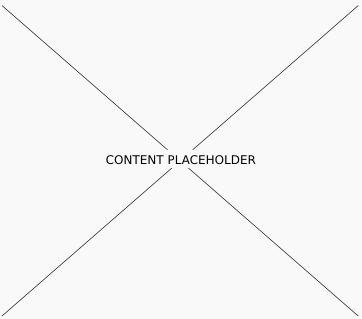
\includegraphics[width=0.9\linewidth]{figures/placeholder.png}
  \caption{Cute picture of robot tying knot}
  \label{fig:frontfig}
\end{figure}

In this paper, we present a solution to the demonstration selection problem that can account for the generalizability of demonstrations and the sequential nature of our applications.
Given a set of demonstrations and a method for generalizing them, we construct a discrete action abstract MDP.
Each action in this MDP is associated with a demonstration and our transition function is defined as applying trajectory transfer to generalize that demonstration.

This construction allows us to learn a Q function from example sequences of state-demonstration pairs.
This is accomplished through a max margin optimization problem whose solution captures the optimality of the examples and the temporal constraints imposed by the sequential nature of our tasks.
Our objective is a linear combination of features which are completely task agnostic and can be applied to any problem where trajectory transfer applies. 
We investigate the utility of this approach in a challenging knot-tieing scenario and show that the greedy application of our learned policy outperforms the nearest-neighbor baseline on a challenging distribution of problems. 
We leverage the fact that we learn a Q function representation of our policy (as opposed to a direct mapping from features to actions) to use a beam search to get near perfect performance in this task.
Finally, we present a method for bootstraping, though a process we call Leave-One-Out-Labelling, that enables us to do Max Margin Q-Learning with no additional human supervision beyond the initial demonstrations.

The rest of this paper is organized as follows: \dhm{fill this in later once we've drafted everything else}


